% ---
% Capítulo 2
% ---
\chapter{Desenvolvimento}


\lettrine[lines=3]{P}{} artindo da utilização de boa parte do projeto efetuado em semestres anteriores, busca-se melhorar todo o funcionamento da placa, tornando-a modular e totalmente programável. Para controlar o que aparecerá no painél, será utilizada uma junção de dois CIs, o 74hc595 e o 74hc138, que receberão a mensagem via ESP32, responsável por fazer a conexão da interface gráfica ate os CIs. O 74hc595 será utilizado como escravo na comunicação SPI. Serial Peripheral Interface ou SPI é um protocolo que permite a comunicação do microcontrolador com diversos outros componentes, formando uma rede. É uma especificação de interface de comunicação série síncrona usada para comunicação de curta distância, principalmente em sistemas embarcados. Dessa forma, o sinal é enviado para todos os LEDs a partir de só um microcontrolador. Já o 74hc198 transmite o sinal para o LED que precisa ser ligado. 

O projeto passará por testes no software Proteus, onde serão analisadas questões como o comportamento de alguns componentes, e também o funcionamento da programação em meio a utilização do circuito e após isso será iniciada a fase de desenvolvimento da PCI. Com relação a programação, serão utilizados dois tipos de linguagem, "C++" para a ESP32 e "python" pra o software Glade, onde será desenvolvida a interface gráfica que permitira a edição dos textos do painél.

Abaixo podemos ver algumas figuras do projeto de semestres passados, que mostram os esquemáticos no proteus(figura \ref{fig:PCB}), e módulo de LEDs(figura \ref{fig:modulo}) .


		\begin{figure}[H]
			\centering\footnotesize
			\caption{PCB e esquema no Proteus}
			\begin{center}
			    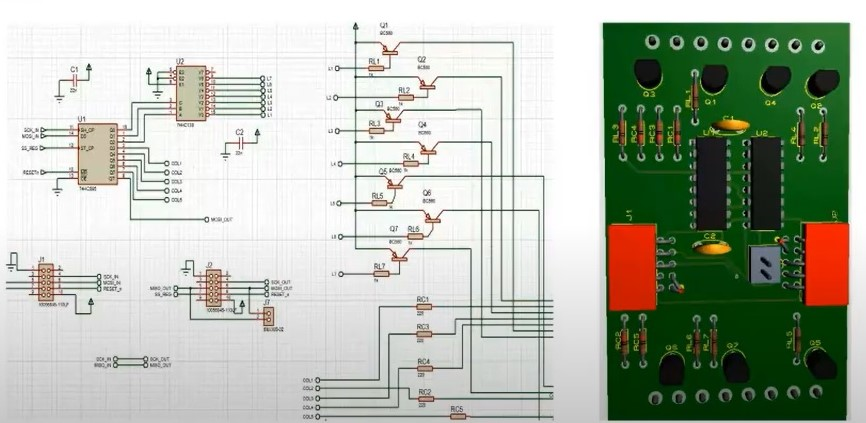
\includegraphics[scale=0.7]{imagens/PCP.jpg}
			\end{center}
			\label{fig:PCB}
			\par Fonte: Arthur Loss, Ivan Correa, Marcelo Junges, Fernanda Brizdo.
		\end{figure}
		\begin{figure}[H]
			\centering\footnotesize
			\caption{Módulos}
			\begin{center}
			    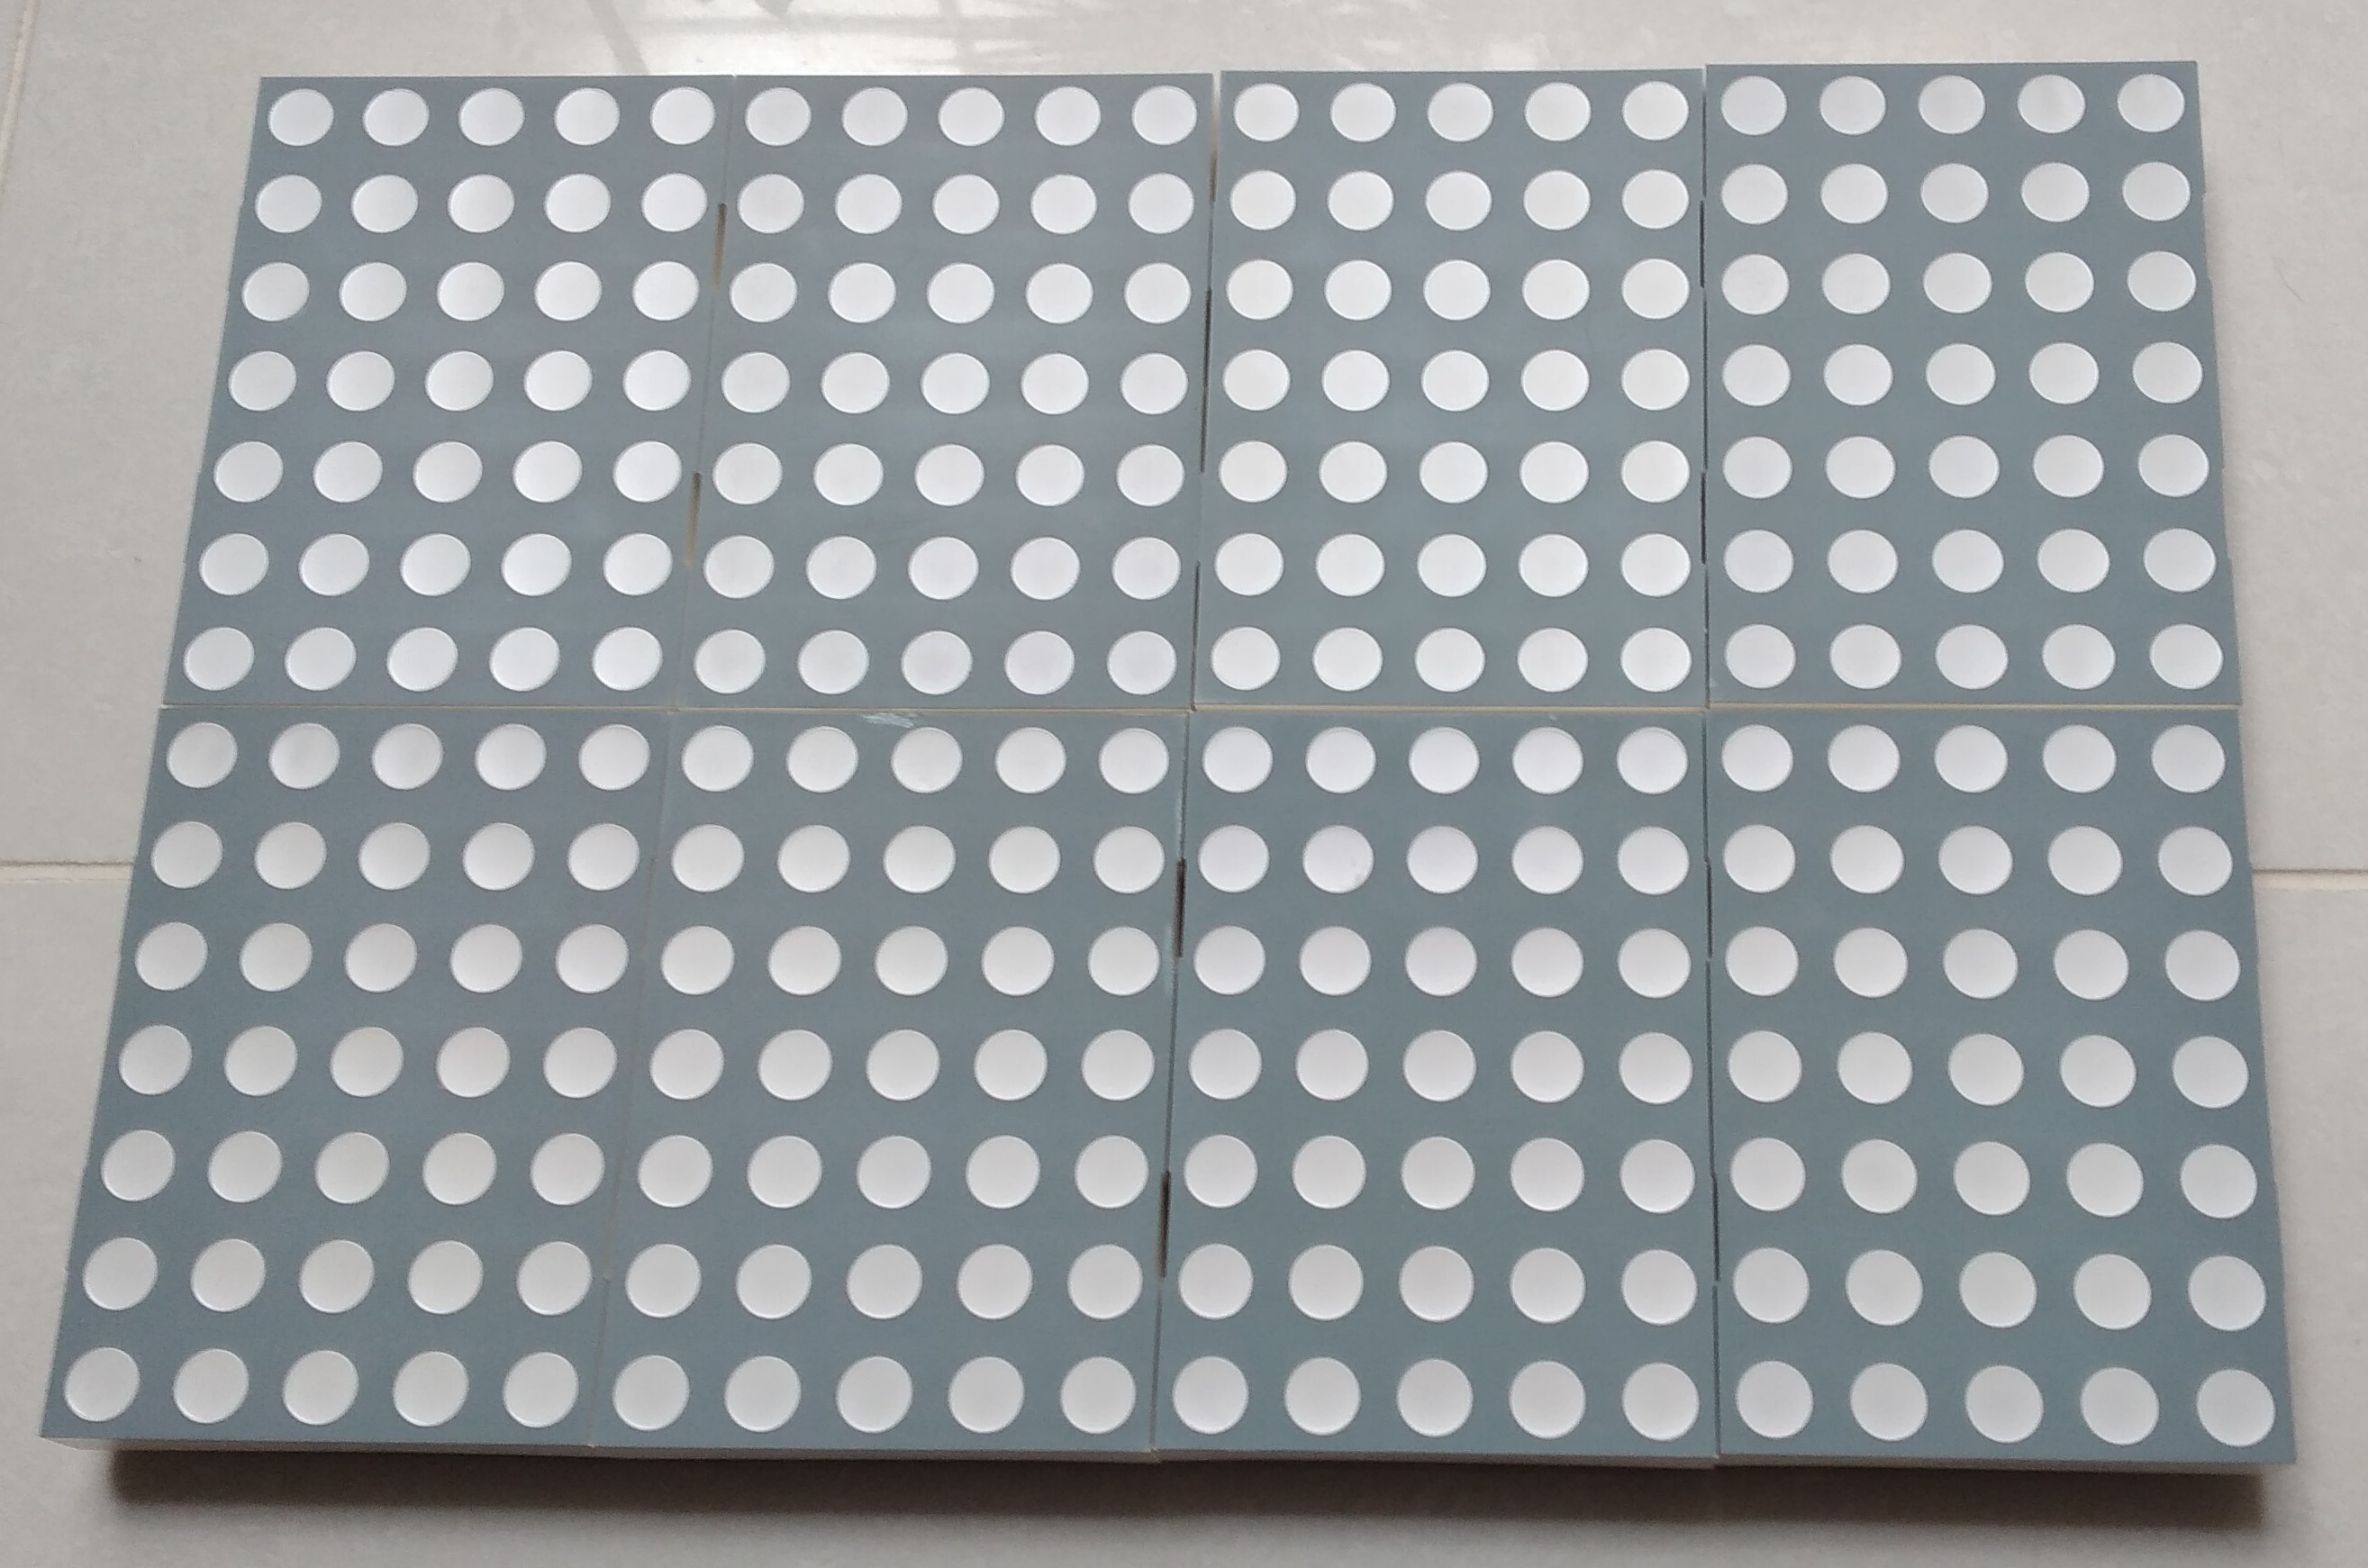
\includegraphics[scale=0.1]{imagens/20210812_111039.jpg}
			\end{center}
			\label{fig:modulo}
			\par Fonte: Edson Melo
		\end{figure}

\section{Itens a serem Adquiridos}

Os componentes implementados no projeto, estão apresentados na Tabela \ref{table:Componentes do projeto}.

\begin{table}[H]
	\centering\footnotesize
	\caption{ Componentes do Projeto Mercado Livre}	
	\begin{tabular}{p{5cm}S[table-format=0.2]S[table-format=0.2]S[table-format=0.2]S[table-format=0.2]S[table-format=0.2]S[table-format=0.2]S[table-format=0.2]}
		\toprule	
		Componentes & {Qtd necessaria} & {Qtd} & {Preço}  & {Link}
		\\
		\midrule
		Módulos de leds & {6} & {10} & {40,50} & \cite{Modulos}\\ 
		BC547 & {42} & {50} & {18,99} & \cite{BC547}\\
		74hc595 & {6} & {10} &{23,74} & \cite{74hc595}\\
		74hc138 & {6} & {10} & {25,42} &\cite{74hc138}\\
		Capacitor 100 nF & {12} & {100} & {28,84}  & \cite{Capacitor100nF}\\
		Conector header 16 pinos 90º & {12} & {10} & {18,90} & \cite{Conectorheader16Pinos}\\
		Conector Latch Fêmea 10 Vias & {12} & {50} & {37,99} & \cite{Conectorlatchfemea}\\ 
		Cabo fita  & {1.27mm/m} & {1} & {18,90} &\cite{CaboFita}\\ 
		Fonte de 5 V 5 A  & {1} & {1} & {32,50} & \cite{Fonte5v}\\
		Esp 32  & {1} & {1} & {42,20} & \cite{Esp32}\\
		Resistores 330 ohms & {42} & {100} & {12,69} & \cite{330}\\
		Resistores 1k ohms & {30} & {100} & {12,49} & \cite{1k}\\
		\bottomrule
	\end{tabular}
	\label{table:Componentes do projeto}
	\par Fonte: Elaborado pelo próprio autor
\end{table}

Também fizemos uma lista em outro site, apresentando valores mais baratos para compra, que estão presentes na tabela abaixo:


\begin{table}[H]
	\centering\footnotesize
	\caption{ Componentes do Projeto Báu da eletrônica}	
	\begin{tabular}{p{5cm}S[table-format=0.2]S[table-format=0.2]S[table-format=0.2]S[table-format=0.2]S[table-format=0.2]S[table-format=0.2]S[table-format=0.2]}
		\toprule	
	Componentes & {Qtd necessaria} & {Qtd} & {Preço}  & {Link}
		\\
		\midrule
		BC547 & {42} & {42} & {15,96} &  \cite{BC547novo}\\
		74hc595 &  {6} & {6} & {13,08} &  \cite{74hc595novo}\\
		74hc138 &  {6} & {6} & {18,42} & \cite{74hc138novo}\\
		Capacitor 100 nF & {12} & {12} & {1,56} & \cite{Capacitor100nFnovo}\\
		Conector header 16 pinos 90º & {12} & {12}& {21,72} &  \cite{Conectorheader16Pinosnovo}\\
		Conector Latch Fêmea 10 Vias & {12} & {12} & {9,36} &  \cite{Conectorlatchfemeanovo}\\ 
		Cabo fita  & {1.27mm/m} & {1} & {4,25} &\cite{CaboFitanovo}\\ 
		Esp 32  & {1} & {1} & {87,40} &  \cite{Esp32novo}\\
		Resistores 330 ohms & {42} & {42} & {2,52} &  \cite{330novo}\\
		Resistores 1k ohms & {30} & {30} & {1,80} & \cite{1knovo}\\
		\bottomrule
	\end{tabular}
	\label{table:Componentes do projeto}
	\par Fonte: Elaborado pelo próprio autor
\end{table}

É importante salientar que alguns componentes como módulo de LEDs, Esp32, cabo fita e resistores, poderão ser providenciados pelo IFSC em conjunto com os professores orientadores. 

\chapter{Cronograma}

O cronograma apresentado na Tabela \ref{table:cronogramaT1} detalha as atividades a serem executadas entre os encontros 8 e 22, exclusivamente, e compreende uma divisão semanal.

\begin{table}[H]
	\centering\footnotesize
	\caption{Cronograma.}	
	\begin{tabular}{p{10cm}S[table-format=0.5]S[table-format=0.5]S[table-format=0.5]S[table-format=0.5]S[table-format=0.2]S[table-format=0.2]S[table-format=0.2]}
		\toprule	
		{Semanas:} & {1} & {2} & {3} & {4} & {5} & {6} & {7}\\
		\midrule
		
		Programar interface gráfica em python(Glade)  &  & X & X &  &  &  &  \\
		Estudo sobre os CIs &  &  & X & X &  &  &\\
		Teste da comunicação SPI    &  &  &  &  & X & X &  \\ 
		Enviar mensagens estáticas no modulo de LEDs   &  &  &  &  &  & X & X \\
		Montagem em matriz de contato & & & & & & & X\\
		\bottomrule
	\end{tabular}
	\label{table:cronogramaT1}
	\par Fonte: Elaborado pelo próprio autor
\end{table}		